\documentclass{article}
\usepackage{graphicx}
\begin{document}

\begin {titlepage}
    \begin{center}
   \line(1,0){200} \\
    \huge{\bfseries MyMoney App}\\
    \line (1,0) {100} \\
    [1.5cm]
    \textsc{\LARGE Comp354}\\
    [1cm]
    \textsc{\large PB-PJ}\\
    [3 cm]
    %by family name by alphabetical order 
    \textsc{\large Matthew Ferderber, Matthew Dugal, Mylene Haurie, Viktoriya Malinova, Eric Morgan, Artem Khomich, \break Kai Nicoll-Griffith, Maximilien Malderle }\\
    [6cm]
    \textsc{\large February 2018}\\

    \end{center}
\end{titlepage}

\fontsize{11pt}{13pt}\selectfont
\setlength{\parindent}{13 pt}

\newpage
 \section {Revision History}
 \paragraph{\indent any big changes done in how the project is set up}
 
\newpage
\tableofcontents


\newpage
\section {Project Description}

\subsection{Introduction}
\paragraph{\indent MyMoney is a desktop application that targets young adults organize and helps them analyse their financial data. The app relies on a user input of data, and can considers multiple accounts at the same time in its analysis. The main end goal of MyMoney is to help visually and statistically represent whether a person is making enough money for its expenses and show which fields of expenses (e.g. eating out, beverages, clothes shopping, house necessities, etc.) is most costly and what percentage of the budget it currently uses up. The app analyses these statistics based on a monthly cycle of expenditures and can alert when a person is spending more money they can afford in a given cycle. }

\subsection{Context}
\paragraph{\indent For iteration 1, we look mainly at transactions. Our app is centered around the idea that each customer class will have one or many bank accounts which can be of any type (ex. Savings, Checking, etc.). The customer class can add transactions for each of its accounts which hold a certain value (if positive, we have a deposit; if negative, we have a withdrawer). The customer class holds a name and a unique ID.}

\subsection{Business Goals}
\paragraph{\indent The business wants to offer an application, which will keep track of the fluctuations in the users funds.  It will determine the inflow and outflow of money on a set period of time.  This will generate information allowing the application to suggest which accounts to use and how much spending is realistic.  The application will be able to account for fixed cyclical expenditures such as rent or many different forms of interest and principal payments.  The principal function of the application will be to help users to achieve their own personal goals in respect to their financial standing.\newline \newline Markets in this industry are rapidly moving online.  The benefits of this, is that products are available to huge amounts of potential customers. The internet also allows for a level of communication, between many different institutions giving the application the ability to analyze saving and saving habits.  This trend is optimal for the sort of product that the business is going to offer. The business is going to target students and young professionals.  The reason being, that this segment is the most tech savvy portion of the population, with no guarantee of long term financial security.  They are most likely to quickly adopt and benefit from the product.   
}

\subsubsection{Competitors and type of competition:}
\paragraph{\indent According to internet searches there are roughly 20 companies that offer money managing applications. These companies can be seen as direct competition, due to the similarity of the service.  The main areas of competition will be to fight for visibility.  With many other competing services how will potential users be educated about the benefits of our platform. Another problem that the business faces in this industry is selecting a revenue model.  The majority of the current money managing services are free to the users and make revenue by selling user information to financial institutions.  Other competitors make a one time charge for the application ranging from $5 to $60.  The third and least popular option is a subscription model, which is only used by one of the companies.}  

\subsubsection{Competitor’s Strengths and Weaknesses:}
\paragraph{\indent The major player is Mint.com owned by Intuit, with roughly 20 million users.  This company has 35 employees and the financial backing of a company with a market cap of 42 B.  This pre existing structure allows the company to have a team of people that have experience in the field since 2006.  They also have a huge support system, allowing the company to find and hire new employees.  This system also allows the competition to have access to funds and marketing firms.  The potential weakness of these businesses is that they already have a fixed application on the market which is being used by customers.  This means that they are not flexible in offering new features that may not be implemented on the pre-existing structure very easily.}


\subsubsection{Competitive advantage:}
\paragraph{\indent The advantage of the business is that the market is not too over saturated and there are enough businesses to gauge which features are more popular than others.  This gives the application enough flexibility to try and tackle a problem the other companies have not solved yet.  This differentiation if properly marketed can be the deciding factor between succeeding and failing.}

\subsubsection{Customers:}
\paragraph{\indent The customers that this application is trying to target are mainly young adults who are either studying or just starting out in the job market.  This segment of the population is on average more tech savvy, making them more likely to adopt the application.  This segment is also not established financially or mature, meaning they may not have a guaranteed income for years to come.  They are also more likely to be unexperienced with financial instruments such as loans, lines of credit or interest in general.  This app will help this segment falling into a credit trap, which can virtually handicap an individual for many years.}

\subsubsection{Suppliers:}
\paragraph{\indent There will be a demand for servers to host the application, and as the user base increases so will the requirement for more computing power.  Due the nature of internet business not many vendors will be involved with the day to day operations, reducing the need for an elaborate supply chain.}

\subsubsection{Advertising & promotion:}
\paragraph{\indent The application will be marketed using a no cost/no subscription model, the goal is to offer a service that is free of charge.  The only income we plan on generating is from fees that will be applied whenever the algorithm increases the savings of the user.  The strategy is that people will have nothing to lose and will only pay from the gains that they earned through the service.  This will incentives people to try out the application, because there is literally nothing to lose.  From this core philosophy advertisers will be able to differentiate the product, because no other company does this.  The datamining aspect of the competitors can be implemented as well.}

\subsubsection{Funding:}
\paragraph{\indent At the beginning the company will focus on acquiring funds from White Knights or Venture Capitalists.  In this domain banks will not lend funds due to the risky nature of the industry.  The business is also to immature to be listed on an exchange.  As the business progresses and profitability is proven, the business plans on attracting the attention of a larger financial institution or tech orientated corporations, to either purchase the business or to offer financial support.}

\subsubsection{Conclusion:}
\paragraph{\indent The main goal of our business is to introduce  a competitive and well differentiated product into the market.  The business is looking to provide a high quality product that will with high probability save the users money.  The sweet of features and the distinct revenue model will differentiate the product in a developing market , leading to hopeful revenues.}

\subsection{Scope}
\paragraph{\indent MyMoney is a three-month long project that aims to deliver a finance-analysing application.  By end of iteration 1, the app should be able to support separate accounts linked to an individual, to have functional and user interactive sections where the client can submit data and… Iteration 2 will take 3 weeks and will support statistical analysis. Iteration 3 will take 2 weeks and will put in place money generating advertisement. }

\subsection{Domain Model}


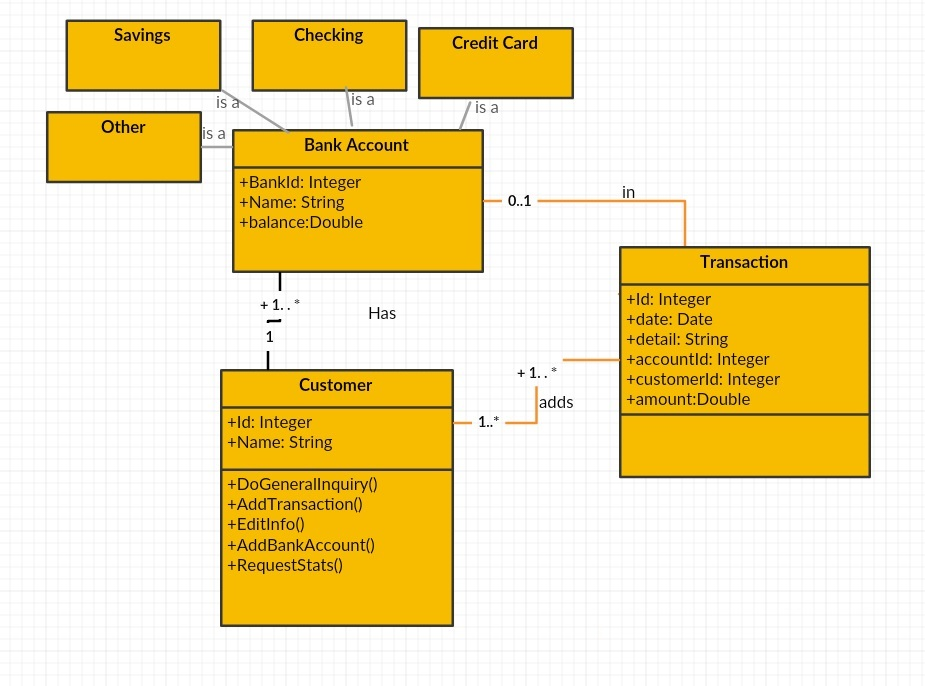
\includegraphics[width=12.5cm]{dm.jpg}
\caption{Figure 1: MyMoney Domain Model}




\subsection{Actors}
\paragraph{\indent There are several important actors that will interact with our application perpetually. The most important ones worth considering are the client, the stakeholders, the business manager(s), coders and the testers.}

\subsubsection{Client}
\paragraph{\indent The client (or user) uses the system for the service it offers. He or she may use all or some of the features of the program, namely data entry, analysis of finances, budget reminders, etc. Clients will also view and click the ads which will generate revenue. Their feedback may help fix missed bugs during the testing stage or give direction to features the app is missing.  }

\subsubsection{Stakeholder}
\paragraph{\indent Similarly to clients, stakeholder may wish to have an account app to view what their investment looks like after an update or at any other given moment. Based on their observations and interactions with the app, they may inform the business manager the changes they want or the direction they wish the app will take in a future iteration.}

\subsubsection{Project Manager}
\paragraph{\indent He or she will interact with the app and will deal with feedback of the clients that he or she will investigate with his team and will report to coders. He or she may also train new employees and help them get familiar with using the app. As the company grows, we may get more than one business manager, and the quantity of interaction a given manager will have with the app will depend on which sector of the company he or she is managing.}

\subsubsection{Coder}
\paragraph{\indent At the very least, the coders and maintenance staff will have to be familiar with the app to be able to do changes, updates and work on future iterations. They may do testing as they code develops to fix bugs or other problems that may emerge along the way.}

\subsubsection{Tester}
\paragraph{\indent They will put the app through a variety of tests at various points of development due to the test-driven nature of development for this project. After each iteration, they will interact with the final product looking for bugs or inaccuracies in the interface of the program and give feedback based on their observations to the coders.}

\newpage
\section {Functional Requirements}
Technical functionality, what the program does/will do

\subsection{Overview}
\subsection{Use cases}
\subsection{Business Rules}

\newpage
\section {Non-Functional Requirements}
HOW the program functions/will function (performance, reliability, etc)

\subsection{Usability}
\subsection{Reliability}
\subsection{Responsiveness}
\subsection{Flexibility}

\newpage
\section {Design Constraints}

\subsection{Time}
\paragraph{ \indent As a student project, one of the primary restraints is time. Due to the majority of team members being full time students, the scope of the project has to be limited to one that is comfortably feasible within the time frame of the semester in accordance with responsibilities the team has to other courses.}

\subsection{Team Size}
\paragraph{\indent Another constraint is team size. Due to the variety of positions that must be filled, we will only have about 3 programmers at a time. In combination with the aforementioned time constraints, we must limit the functionality of our program to the what we determine are the essential features, and then expand on them as time permits.}

\subsection{Software}
\paragraph{\indent In accordance with the requirements laid out in the project description, the program must be a desktop application developed in Eclipse using Java, and make use of one of Java's GUI packages. Additionally, we are required to use GitHub to maintain and iterate upon our design and LaTeX for documentation. The documentation will also require we utilize UML modeling software to input diagrams when appropriate. Because we must have a way to store and track all of the user's financial information, we also must utilize an SQL database.}

% Not sure if this is a bit redundant with the Software sections,so feel free to delete
\subsection{Knowledge}
\paragraph{\indent Many of the softwares and some of the coding languages we currently work with are unfamiliar to members of the team. Attending crash tutorials and reviewing online resources in an attempt to fill in the knowledge gaps is both time consuming and cognitively tiring when it is in such concentration. Slack, GitHub and LaTeX all presented us with a learning curve and we still have not discovered all the features that these indispensable tools offer us.  }

\subsection{Budget}
\paragraph{\indent The budget is also a constraint, or more accurately, the lack of one is. As a class project, we are not developing the software under contract or financial limitations, which means it all is being developed on the hardware and software already available to us.}


\newpage
\section {Glossary}

\textbf{\indent Eclipse: }An integrated development environment used for programming mainly in Java. It is one of the most popular of its kind.\\

\textbf{GitHub: }Version control system that keeps all changes in a project up-to-date while multiple people work on it simultaneously \\

\textbf{GUI: }Short for graphical user interface. This interface represents what the end user sees and allows the user to interact with the system without needing to code commands. \\

\textbf{Iteration: }A cycle consisting of design, development and testing of a new feature that is ultimately added in a overall application\\

\textbf{LaTeX: }Document preparation software used mainly for scientific and academic documents.\\

\textbf{Slack: }Online collaboration app based heavily on compartmentalized instant messaging.\\

\textbf{SQL database: }SQL, short of structured query language, is a language used to manipulate databases. A SQL database is a database which is accessed through this specific programming language.\\

\textbf{Test-driven project:}A project that is driven by different tests put in place before coding even starts. The goal is that the end product passed these tests that were set from the start.\\

\textbf{UML modeling: }A visual representation of the main classes, attributes and methods composing an application, website or other code-based product.\\


\newpage
\begin{thebibliography}{9}

\bibitem{source} 
Computer Hope. "GUI," \textit{Computer Hope}, Oct. 30 2017. [Online]. Available: https://www.computerhope.com/jargon/g/gui.htm. [Accessed: Jan. 31,2018].

\bibitem{source} 
JCG. "JavaFX ListView Example," \textit{Java Code Geeks}, March 15, 2o16. [Online]. Available: https://examples.javacodegeeks.com /desktop-java/javafx/listview-javafx/javafx-listview-example/. [Accessed: Jan. 28,2018].

\bibitem{source} 
K. Brown. "What Is GitHub, and What Is It Used For?," \textit{How-To Geek}, Sept. 21 2016. [Online]. Available: https://www.howtogeek.com/180167/htg- explains-what-is-github-and-what-do-geeks-use-it-for/. [Accessed: Jan. 28,2018].

\bibitem{source} 
M. Mansfield. "What is Slack and How Do I Use It for My Team?," \textit{Small Business Trends}, June 7, 2016. [Online]. Available: https://smallbiztrends.com/2015/12/slack-use-team.html. [Accessed: Jan. 31,2018].

\bibitem{source} 
Oracle. "Introduction to FXML," \textit{Oracle}, June 21, 2008. [Online]. Available: https://docs.oracle.com/javafx/2/api/javafx/fxml/doc-files/introduction\_to\_fxml.html. [Accessed: Jan. 28,2018].

\bibitem{source} 
Oracle. "Packages," \textit{Oracle}, 2014. [Online]. Available: https://docs.oracle.com/javafx/2/api/overview-summary.html. [Accessed: Jan. 28,2018].

\bibitem{source} 
Oracle. "Skinning JavaFX Applications with CSS," \textit{Oracle}, June 2013. [Online]. Available: https://docs.oracle.com/javafx/2/css\_tu torial/jfxpub-css\_tutorial.htm. [Accessed: Jan. 28,2018].

\bibitem{source} 
Refsnes Data. "Introduction to SQL," \textit{w3schools.com}, 2018. [Online]. Available:https://www.w3schools.com/sql/sql\_intro.asp. [Accessed: Jan. 31,2018].

\bibitem{source} 
The LaTeX Project Public. "LaTeX – A document preparation system," \textit{The LATEX Project}. [Online]. Available: https://www.latex-project.org/. [Accessed: Jan. 31,2018].







\end{thebibliography}
\addcontentsline{toc}{section}{References}

 
\end {document}

